%%%%%%%%%%%%%%%%%%%%%%%%%%%%%%%%%%%%%%%%%%%%%%%%%%%%%%%%%%
%   Autoren:
%   Prof. Dr. Bernhard Drabant
%   Prof. Dr. Dennis Pfisterer
%   Prof. Dr. Julian Reichwald
%%%%%%%%%%%%%%%%%%%%%%%%%%%%%%%%%%%%%%%%%%%%%%%%%%%%%%%%%%

%%%%%%%%%%%%%%%%%%%%%%%%%%%%%%%%%%%%%%%%%%%%%%%%%%%%%%%%%%
%	ANLEITUNG: 
%   1. Ersetzen Sie firmenlogo.jpg im Verzeichnis img
%   2. Passen Sie alle Stellen im Dokument an, die mit 
%      @stud 
%      markiert sind
%%%%%%%%%%%%%%%%%%%%%%%%%%%%%%%%%%%%%%%%%%%%%%%%%%%%%%%%%%

%%%%%%%%%%%%%%%%%%%%%%%%%%%%%%%%%%%%%%%%%%%%%%%%%%%%%%%%%%
%	ACHTUNG: 
%   Für das Erstellen des Literaturverzeichnisses wird das 
%   modernere Paket biblatex in Kombination mit biber 
%   verwendet - nicht mehr das ältere Paket BibTex!
%
%   Bitte stellen Sie Ihre TeX-Umgebung entsprechend ein (z.B. TeXStudio): 
%   Einstellungen --> Erzeugen --> Standard Bibliographieprogramm: biber
%%%%%%%%%%%%%%%%%%%%%%%%%%%%%%%%%%%%%%%%%%%%%%%%%%%%%%%%%%

\documentclass[fontsize=11.4pt,BCOR=3mm,DIV=12,parskip=half,listof=totoc,
               paper=a4,toc=bibliography,pointlessnumbers]{scrreprt}
               
               %toc=listof,listof=entryprefix,
               
\makeindex

%% Elementare Pakete, Konfigurationen und Definitionen werden geladen (gegebenenfalls anpassen)
% !TEX root =  master.tex

%%%%%%%%%%%%%%%%%%%%%%%%%%%%%%%%%%%%%%%%%%%%%%%%%%%%%%%%%%%%%%%%%%
%	ANLEITUNG: 
% Passen Sie gegebenenfalls alle Stellen im Dokument an, die mit 
% @stud 
% markiert sind.
%%%%%%%%%%%%%%%%%%%%%%%%%%%%%%%%%%%%%%%%%%%%%%%%%%%%%%%%%%%%%%%%%%

\usepackage{makeidx}                  % allows index generation
\usepackage{listings}	                %Format Listings properly
\usepackage{lipsum}                   % Blindtext
\usepackage{graphicx}                 % use various graphics formats
\usepackage[german]{varioref}         % nicer references \vref
\usepackage{caption}	                % better Captions
\usepackage{booktabs}                 % nicer Tabs
\usepackage[hidelinks=true]{hyperref} % keine roten Markierungen bei Links
\usepackage{fnpct}                    % Correct superscripts 
\usepackage{calc}                     % Used for extra space below footsepline, in particular
\usepackage{array}
\usepackage{acronym}
\usepackage{algorithm}
\usepackage{algpseudocode}
\usepackage{setspace}
\usepackage{tocloft}

%% Schriftarten- und Zeichenpakete
\usepackage[T1]{fontenc}
\usepackage[utf8]{inputenc}

%%
%% @stud
%%
%%	FONT SELECTION: Schriftarten und Schriftfamilie
%%%%%%%%%%%%%
%% SCHRIFTART
%%%%%%%%%%%%%
% 0) without decomment: normal font families 
% ...
% 1) Latin Modern 
%\usepackage{lmodern}        
% 2) Times 
%\usepackage{mathptmx}         
% 3) Helvetica
%\usepackage[scaled=.92]{helvet} 
%%%%%%%%%%%%%%%%%%
%%	SCHRIFTFAMILIE
%%%%%%%%%%%%%%%%%%
% ohne Serifen
\renewcommand*{\familydefault}{\sfdefault}
\addtokomafont{disposition}{\sffamily}
%
% mit Serifen
%\renewcommand*{\familydefault}{\rmdefault}
%\addtokomafont{disposition}{\rmfamily}
%
% Typewriter
%\renewcommand*{\familydefault}{\ttdefault}
%\addtokomafont{disposition}{\ttfamily}

%%
%% @stud
%%
%% LANGUAGE SETTINGS
\usepackage[ngerman]{babel} 	        % german language
\usepackage[german=quotes]{csquotes} 	% correct quoting using \enquote{}
%\usepackage[english]{babel}          % english language
%\usepackage{csquotes} 	              % correct quoting using \enquote{}

%%
%% @stud
%%
%% Uncomment the following lines to support hard URL breaks in bibliography 
%\apptocmd{\UrlBreaks}{\do\f\do\m}{}{}
%\setcounter{biburllcpenalty}{9000}% Kleinbuchstaben
%\setcounter{biburlucpenalty}{9000}% Großbuchstaben

%%
%% @stud
%%
%% FOOTNOTES: Count footnotes over chapters
%% \counterwithout{footnote}{chapter}

%	ACRONYMS
\makeatletter
\@ifpackagelater{acronym}{2015/03/20}
{\renewcommand*{\aclabelfont}[1]{\textbf{{\acsfont{#1}}}}}{}
\makeatother

%	LISTINGS
% @stud: ggf. Namen/Text anpassen (englisch)
\renewcommand{\lstlistingname}{Quelltext} 
\renewcommand{\lstlistlistingname}{Quelltextverzeichnis}
\lstset{numbers=left,
	numberstyle=\tiny,
	captionpos=b,
	basicstyle=\ttfamily\small}

%	ALGORITHMS
% @stud: ggf. Namen/Text anpassen (englisch)
\renewcommand{\listalgorithmname}{Algorithmenverzeichnis}
\floatname{algorithm}{Algorithmus}

%	PAGE HEADER / FOOTER
%	Warning: There are some redefinitions throughout the master.tex-file!  DON'T CHANGE THESE REDEFINITIONS!
\RequirePackage[automark]{scrlayer-scrpage}
%alternatively with separation lines: \RequirePackage[automark,headsepline,footsepline]{scrlayer-scrpage}

\renewcommand{\chaptermarkformat}{}
\RedeclareSectionCommand[beforeskip=0pt]{chapter}
\clearscrheadfoot

%\ifoot[\rule{0pt}{\ht\strutbox+\dp\strutbox}DHBW Mannheim]{\rule{0pt}{\ht\strutbox+\dp\strutbox}DHBW Mannheim}
\ofoot[\rule{0pt}{\ht\strutbox+\dp\strutbox}\pagemark]{\rule{0pt}{\ht\strutbox+\dp\strutbox}\pagemark}
\ohead{\headmark}

\newcommand{\TitelDerArbeit}[1]{\def\DerTitelDerArbeit{#1}\hypersetup{pdftitle={#1}}}
\newcommand{\AutorDerArbeit}[1]{\def\DerAutorDerArbeit{#1}\hypersetup{pdfauthor={#1}}}
\newcommand{\Firma}[1]{\def\DerNameDerFirma{#1}}
\newcommand{\Kurs}[1]{\def\DieKursbezeichnung{#1}}
\newcommand{\Abteilung}[1]{\def\DerNameDerAbteilung{#1}}
\newcommand{\Studiengangsleiter}[1]{\def\DerStudiengangsleiter{#1}}
\newcommand{\WissBetreuer}[1]{\def\DerWissBetreuer{#1}}
\newcommand{\FirmenBetreuer}[1]{\def\DerFirmenBetreuer{#1}}
\newcommand{\Bearbeitungszeitraum}[1]{\def\DerBearbeitungszeitraum{#1}}
\newcommand{\Abgabedatum}[1]{\def\DasAbgabedatum{#1}}
\newcommand{\Matrikelnummer}[1]{\def\DieMatrikelnummer{#1}}
\newcommand{\Studienrichtung}[1]{\def\DieStudienrichtung{#1}}
\newcommand{\ArtDerArbeit}[1]{\def\DieArtDerArbeit{#1}}
\newcommand{\Hochschule}[1]{\def\Hochschule{#1}}
\newcommand{\Literaturverzeichnis}{Literaturverzeichnis}

\newcommand{\settingBibFootnoteCite}{
	\setlength{\bibparsep}{\parskip}		  % Add some space between biblatex entries in the bibliography
	\addbibresource{bibliography.bib}	    % Add file bibliography.bib as biblatex resource
	\DefineBibliographyStrings{ngerman}{andothers = {{et\,al\adddot}},}
}

\newcommand{\setTitlepage}{
	% !TEX root =  master.tex
% @stud: ggf. Namen/Text anpassen (englisch)
\begin{titlepage}
\begin{minipage}{\textwidth}
		\vspace{-2cm}
		\noindent 
\includegraphics[scale=0.5]{\imagedir/VoBaBKLogo.jpg} \hfill 
\includegraphics{\imagedir/CAS-Logo.jpg}
\end{minipage}
\vspace{1.5em}
%\sffamily
\begin{center}
	{\textsf{\large Duale Hochschule Baden-W\"urttemberg - CAS}}\\[4em]
	{\textsf{\textbf{\large{\DieArtDerArbeit}}}}\\[6mm]
	{\textsf{\textbf{\Large{}\DerTitelDerArbeit}}} \\[15mm]
	{\textsf{\textbf{\large{}Studiengang Wirtschaftsinformatik}}\\[6mm]
	}\vspace{10em}
	
	\begin{minipage}{\textwidth}
		\begin{tabbing}
		Wissenschaftliche(r) Betreuer(in): \hspace{0.85cm}\=\kill
		Verfasser(in): \> \DerAutorDerArbeit \\[1.5mm]
		Matrikelnummer: \> \DieMatrikelnummer \\[1.5mm]
		Firma: \> \DerNameDerFirma  \\[1.5mm]
		Abteilung: \> \DerNameDerAbteilung \\[1.5mm]
		Kurs: \> \DieKursbezeichnung \\[1.5mm]
		Studiengangsleiter: \> \DerStudiengangsleiter \\[1.5mm]
		Wissenschaftliche(r) Betreuer(in): \> \DerWissBetreuer \\[1.5mm]
		Firmenbetreuer(in): \> \DerFirmenBetreuer \\[1.5mm]
		Bearbeitungszeitraum: \> \DerBearbeitungszeitraum\\[1.5mm]
%		alternativ:\\[1.5mm]
%		Eingereicht: \> \DasAbgabedatum	
		\end{tabbing}
	\end{minipage}
\end{center}
\end{titlepage}
	\pagenumbering{roman} % Römische Seitennummerierung
	\normalfont	
}

\newcommand{\initializeText}{
	\clearpage
	\ihead{\chaptername~\thechapter} % Neue Header-Definition
	\pagenumbering{arabic}           % Arabische Seitenzahlen
}

\newcommand{\initializeBibliography}{
	\ihead{}
	\printbibliography[title=\Literaturverzeichnis] 
	\cleardoublepage
}

\newcommand{\initializeAppendix}{
	\appendix
  \ihead{}
  \cftaddtitleline{toc}{chapter}{Anhang}{}
}



%%
%% @stud
%%
%% PERSÖNLICHE ANGABEN (BITTE VOLLSTÄNDIG EINGEBEN zwischen den Klammern: {...})
%%

%% Arbeit Individuell
\ArtDerArbeit{Forschungsprojektarbeit 1} % "Bachelor" oder "Projekt" wählen
\TitelDerArbeit{Optimierung von Testkapazitäten durch PCR-Pooling}
\WissBetreuer{Prof. Dr. Martin}
\Bearbeitungszeitraum{14.12.2021 -- 14.02.2022}
\Abgabedatum{14.12.2022}

%% Hochschule
\Kurs{Wirtschaftsinformatik}
\Studiengangsleiter{Prof. Dr. Martin, Prof. Dr. Kessel}

%% Student
\AutorDerArbeit{Daniel Jacobi}
\Matrikelnummer{8041730}

%% Firma
\Firma{Volksbank Backnang eG}
\Abteilung{Marktfolge Aktiv - Firmenkunden}
\FirmenBetreuer{Herr Stephan Denz}

%%
%% @stud
%%
%% BIBLIOGRAPHY (@stud: Bibliographie-Stil wählen - Position und Indizierung)
%%  Auswahl zwischen: 
%%   NUMERIC Style
%%   IEEE Style
%%   ALPHABETIC Style
%%   HARVARD Style
%%   CHICAGO Style 
%%   (oder eigenen zulässigen Stil wählen) 
%%
%%%%%%%%%%%%%
%% Zitierstil
%%%%%%%%%%%%%
% NUMERIC Style - e. g. [12]
%\newcommand{\indextype}{numeric} 
%
% IEEE Style - numeric kind of style 
%\newcommand{\indextype}{ieee} 
%
% ALPHABETIC Style - e. g. [AB12]
%\newcommand{\indextype}{alphabetic} 
%
% HARVARD Style 
%\newcommand{\indextype}{apa} 
%
% CHICAGO Style 
%\newcommand{\indextype}{authoryear}
%
%%%%%%%%%%%%%%%%%%%%%%
%% Position des Zitats
%%%%%%%%%%%%%%%%%%%%%%
%\newcommand{\position}{inline} 
%
% (!!) FOOTNOTE POSITION NOT RECOMMENDED IN MINT DOMAIN:
%\newcommand{\position}{footnote}

%% Final: Setzen des Zitierstils und der Zitatposition
\usepackage[
backend=biber,
autocite=footnote,
bibstyle=apa, %Kopiert von RP
style=apa
]{biblatex} 	
\settingBibFootnoteCite
\addbibresource{bibliography.bib} %Kopiert von RP

\usepackage{wrapfig}
\usepackage{subfig}
\usepackage{helvet}

%%
%% Definitionen und Commands
%%
\newcommand{\abs}{\par\vskip 0.2cm\goodbreak\noindent}
\newcommand{\nl}{\par\noindent}
\newcommand{\mcl}[1]{\mathcal{#1}}
\newcommand{\nowrite}[1]{}
\newcommand{\NN}{{\mathbb N}}
\newcommand{\imagedir}{img}

\makeindex

\begin{document}

\setTitlepage

%%%%%%%%%%%%%%%%%%%%%%%%%%%%%%%%%%%
% EHRENWÖRTLICHE ERKLÄRUNG
%
% @stud: ewerkl.tex bearbeiten
%
% !TEX root =  master.tex
\clearpage
\chapter*{Ehrenwörtliche Erklärung}

% Wird die folgende Zeile auskommentiert, erscheint die ehrenwörtliche
% Erklärung im Inhaltsverzeichnis.

% \addcontentsline{toc}{chapter}{Ehrenwörtliche Erklärung}
Ich versichere hiermit, dass ich die vorliegende Arbeit mit dem Titel ``\textit{\DerTitelDerArbeit}'' selbstständig verfasst und 
keine anderen als die angegebenen Quellen und Hilfsmittel benutzt habe. Ich versichere zudem, dass die eingereichte elektronische 
Fassung mit der gedruckten Fassung übereinstimmt.

\vspace{3cm}
Heilbronn, 14.02.2022 \hfill \DerAutorDerArbeit
 
\cleardoublepage  
%%%%%%%%%%%%%%%%%%%%%%%%%%%%%%%%%%%

%%%%%%%%%%%%%%%%%%%%%%%%%%%%%%%%%%%
% SPERRVERMERK
%
% @stud: nondisclosurenotice.tex bearbeiten
%
%% !TEX root =  master.tex
\chapter*{Sperrvermerk}

\begin{center}
\fbox{
		\begin{minipage}{33em}
			\textbf{Ein Sperrvermerk sollte nur bei berechtigtem Bedarf gesetzt werden!\\[10pt] 
				Beachten Sie, dass mit Sperrvermerk	versehene Arbeiten nicht für weitere wissenschaftliche Zwecke 
				außerhalb des Firmenkontextes oder zur Publikation verwendet werden dürfen.\\[10pt]
				Wir empfehlen, wenn m\"oglich, auf den Sperrvermerk zu verzichten.\\[10pt]
				Besprechen Sie diese Problematik mit Ihrer Firma!}
		\end{minipage}
}
\end{center}

(Mustertext) Der Inhalt dieser Arbeit darf weder als Ganzes noch in Auszügen Personen außerhalb des Prüfungsprozesses 
und des Evaluationsverfahrens zugänglich gemacht werden, sofern keine anders lautende Genehmigung der Ausbildungsstätte vorliegt. 

\cleardoublepage
 
%\cleardoublepage
%%%%%%%%%%%%%%%%%%%%%%%%%%%%%%%%%%%

%%%%%%%%%%%%%%%%%%%%%%%%%%%%%%%%%%%
%	KURZFASSUNG
%
% @stud: acknowledge.tex bearbeiten
%
%% !TEX root =  master.tex
\chapter*{Danksagung}

Hier können Sie eine Danksagung schreiben. 



%\cleardoublepage 
%%%%%%%%%%%%%%%%%%%%%%%%%%%%%%%%%%%

%%%%%%%%%%%%%%%%%%%%%%%%%%%%%%%%%%%
% VERZEICHNISSE und ABSTRACT
%
% @stud: ggf. nicht benötigte Verzeichnisse auskommentieren/löschen
%
\tableofcontents
\cleardoublepage

% Abbildungsverzeichnis
\phantomsection
\addcontentsline{toc}{chapter}{\listfigurename}
\listoffigures
\cleardoublepage

%	Tabellenverzeichnis
%\phantomsection
%\addcontentsline{toc}{chapter}{\listtablename}
%\listoftables
%\cleardoublepage

%	Listingsverzeichnis / Quelltextverzeichnis
%\lstlistoflistings
%\cleardoublepage

% Algorithmenverzeichnis
%\listofalgorithms
%\cleardoublepage

% Abkürzungsverzeichnis
% @stud: acronyms.tex bearbeiten
%% !TEX root =  master.tex
\clearpage
\chapter*{Abkürzungsverzeichnis}	
\addcontentsline{toc}{chapter}{Abkürzungsverzeichnis}

\begin{acronym}[XXXXXXX]
	\acro{Schnelltest}[Schnelltest]{Rapid Antigen whatever... TODO}
	\acro{PCR}[PCR]{polymerase chain-reaction}

\end{acronym} 
%\cleardoublepage

%	Kurzfassung / Abstract
% @stud: abstract.tex bearbeiten
% !TEX root =  master.tex
\chapter*{Kurzfassung (Abstract)}
\addcontentsline{toc}{chapter}{Kurzfassung (Abstract)}

Hier können Sie die Kurzfassung (engl.~Abstract) der Arbeit schreiben. Beachten Sie dabei die Hinweise zum Verfassen der Kurzfassung.


 
\cleardoublepage

%%%%%%%%%%%%%%%%%%%%%%%%%%%%%%%%%%%%%%%%%%%%%%%%%%%%%%%%%%%%%%%%%%%%%%%%%%%%%%%%%%%%%%%%%%
% KAPITEL UND ANHÄNGE
%
% @stud:
%   - nicht benötigte: auskommentieren/löschen
%   - neue: bei Bedarf hinzufügen mittels input-Kommando an entsprechender Stelle einfügen
%%%%%%%%%%%%%%%%%%%%%%%%%%%%%%%%%%%%%%%%%%%%%%%%%%%%%%%%%%%%%%%%%%%%%%%%%%%%%%%%%%%%%%%%%%

\initializeText
\onehalfspacing

%%%%%%%%%%%%%%%%%%%%%%%%%%%%%%%%%%%
% KAPITEL
%
% @stud: einzelne Kapitel bearbeiten und eigene Kapitel hier einfügen
%

% Research Proposal einfügen
%% !TEX root =  master.tex

\chapter{Reserch Proposal vom 30.11.2021}
\section{Problemstellung und Forschungsziel}
Der Testung der Bevölkerung ist eine der wichtigsten Maßnahmen zur Pandemiebekämpfung.
Zielführend wäre deshalb, hierbei die ungenauen Antigen-Schnelltests\footnote{WuerzburgStudie}
durch das präziseren PCR-Verfahren\footnote{Polymerase Chain Reaction}
zu ersetzen.
Aktuell ist dies aufgrund der hierfür erforderlichen Laborkapazitäten und hohen Kosten nicht umsetzbar.\footnote{rki-bericht 2021}

Die vorgesehene Arbeit hat zum Ziel, existierende Pooling-Verfahren zu überprüfen.
Die Proben mehrerer Patienten werden hierbei kombiniert und gemeinsam getestet.
Diese Verfahren bieten erhebliche Steigerungspotenziale für die Kapazitäten der PCR-Testungen.\footnote{Aertzeblatt}
Bei der anlasslosen Massentestung könnte hierdurch eine Qualitätssteigerung erreicht werden.
Identifiziert werden soll ein Pooling-Verfahren, welches diese Steigerung ohne signifikanten Qualitätsverlust ermöglicht.
Ziel der Arbeit ist deshalb, Pooling-Methoden nach den folgenden Anforderungen zu prüfen:
\begin{itemize}
	\setlength{\itemsep}{-8pt}
	\item Potenzial zur Erhöhung der Testkapazitäten
	\item Robustheit gegen Fehlanwendung
	\item Risiko von falschen Ergebnissen
	\item Anwendbarkeit im betrieblichen Umfeld
\end{itemize}

Während der Pandemie haben sich viele Forschungsgruppen an Pooling-Verfahren gearbeitet.\footnote{viehweger increased 2020}
Hierbei sind viele unterschiedliche Ansätze entstanden.\footnote{verwilt evaluation 2021}
Die vorliegende Arbeit möchte diese Methoden zunächst analysieren und zu Clustern ähnlicher Verfahren aggregieren.
Anschließend soll  eine Überprüfung auf Effizienz und Robustheit der unterschiedlichen Verfahren stattfinden.
Hierfür sollen eine Simulation oder eine argumentativ-deduktive Analyse eingesetzt werden.

\textbf{Primäres Forschungsziel}\newline
Analyse existierender PCR-Pooling-Verfahren.\newline
Überprüfung dieser Methoden auf Effizienz und Robustheit.

\textbf{Sekundäres Forschungsziel}\newline 
Erarbeitung einer Referenzimplementierung für das betriebliche Umfeld.\newline

\section{Aktueller Stand der Wissenschaft}
\subsection{Das PCR-Testverfahren}
Um die Grundlagen für spätere Kapitel zu legen, soll zunächst die allgemeine Funktionsweise des PCR-Verfahrens erläutert werden.
Die verfahrensüblichen Qualiätsmerkmale Sensitivität und Spezifität werden beschrieben und auf Ablauf sowie Logistik der Testungen eingegangen.

Das PCR-Verfahren existierte bereits vor der COVID-19-Pandemie.
Es wird seit 1983
\footnote{wink pcr 1994}
zur Erkennung von Viruserkrankungen eingesetzt.
Sowohl wissenschaftliche Literatur\footnote{schmidt novel 2020}
als auch praxisnahe Publikationen\footnote{wehrle weber pcr 1994}
sind verfügbar.\footnote{clewley polymerase 1995}
Forschungsrelevante Aussagen zur Wirksamkeit und Fehlerquote der Testung werden hierbei ausschließlich auf Quellen gestützt, welche die wissenschaftlichen Qualitätsstandards erfüllen.
Für betriebswirtschaftliche und ablauforganisatorische Themenbereiche wird die Einbeziehung von praxisnahe Literatur als sinnvoll erachtet.

\subsection{PCR-Pooling-Verfahren}
PCR-Pooling-Verfahren wurden bereits vor der Pandemie zur Diagnose anderen Viruserkrankungen erfolgreich eingesetzt.
\footnote{Aertzeblatt}
Hierbei werden die Proben mehrerer Patienten vermischt, um durch einen gemeinsamen Test den Aufwand zu senken.
Im Laufe der Pandemie wurden von vielen Forschungsgruppen und Laboren Methoden entwickelt, um PCR-Pooling durchzuführen.
\footnote{calabrese how 2021}
Zur Robustheit des PCR-Verfahren gegen Verwässerung der Proben und den Skalierungsmöglichkeiten gibt es widersprüchliche Aussagen.
Einige Methoden empfehlen, dass maximal fünf Personen gemeinsam getestet werden.
\footnote{schmidt novel 2020}
Andere vermischen die Proben von 25-40 Patienten.
\footnote{verwilt evaluation 2021}
Das Ärzteblatt bescheinigt den Blutspendediensten die meiste Erfahrung mit PCR-Pooling-Verfahren.
\footnote{Aertzeblatt}
Um Blutspenden auf HIV und Hepatitis zu testen, kommen Pooling-Verfahren hier seit Jahrzehnten zum Einsatz.

Ein Vergleich dieser Pooling-Studien und der erforschten Methoden wird ein Schwerpunkt dieses Kapitels.
Ein Fokus ist hierbei die Fehleranfälligkeit der Tests bei unterschiedlichen Bedingungen und Verfahren.

Die wissenschaftliche Artikel, welche den Verfahren zugrunde liegen, werden aufgrund der Tagesaktualität teilweise von Pre-Print-Servern stammen.\footnote{viehweger increased 2020}
In diesen Fällen ist noch keinen Peer-Review erfolgt, weswegen diese Quellen besonders kritisch reflektiert und mit anderen Publikationen verglichen werden müssen.\footnote{verwilt evaluation 2021}
Die Einhaltung des wissenschaftlichen Anspruchs wird durch den Vergleich der vielen Publikationen und auf Basis der zugrundeliegenden Literatur sichergestellt.
Eine Validierung und Plausibilisierung der Methoden ist ohnehin im Rahmen der primären Forschungsfrage vorgesehen.

\subsection{Methoden der Kanalcodierung}
Ein Forschungsgebiet der Informatik ist die Integritätsprüfung von Speichern und Signalübertragungen.
Die Forscher entwickeln Algorithmen, für die Erkennung und Berichtigung von Fehlern.\footnote{hamming information 1987}
Die Anforderungen sind hierbei stark abhängig vom Anwendungsfall und der zu erwartenden Fehlerverteilung.\footnote{blahut algebraic 1992}

Dieses Kapitel dient dazu, ein Verständnis für die Funktionsweise unterschiedlicher Codierungsverfahren zu vermitteln.
Anhand von Beispielen werden die Unterschiede und Eigenschaften verschiedener Verfahren aufgezeigt.
Verdeutlicht wird hierdurch, nach welchen Kriterien Codierungsverfahren bewertet und verglichen werden können.
Aus der Kanalcodierung werden Anforderungen, Konzepte und Terminologie\footnote{dankmeier codierung 1994}
für die Analyse der Pooling-Verfahren übernommen.

Die Existenz dieses Kapitels ist noch ungewiss.
Sein Zweck wäre, die theoretische Grundlage für eine argumentativ-deduktive Analyse der Pooling-Methoden zu liefern.
Sollte diese Analyse zugunsten einer Simulation entfallen, ist dieses Kapitel obsolet.\footnote{Vgl. Gliederung der Arbeit}

\section{Forschungsmethodik und Vorgehen}
\subsection{Validierung der Modelle}
Im vorherigen Kapitel wurden anhand von internationalen Studien Verfahren für das PCR-Pooling erarbeitet.
Die ermittelten Modelle sollen in diesem Kapitel durch Forschungsmethoden der Wirtschaftsinformatik validiert werden.

Bei mangelhafter Umsetzung einer Pooling-Methode, könnten die Fehlerrate der Testverfahren steigen oder Proben kontaminiert werden.
Das Ergebnis wären ein Mehraufwand durch erneute Testung oder unentdeckte Fehldiagnosen.
Ziel ist es, eine geeignete Methode und Skalierung zu finden und diese auf Robustheit gegen Fehlern zu überprüfen.
Als Forschungsmethoden für die Validierung sind eine \textbf{Simulation} oder eine \textbf{argumentativ-deduktiven Analyse} vorgesehen.
Hierbei sollen die Grenzen der beschriebenen Verfahren erforscht werden.

Getestet werden sollen beispielsweise:
\begin{itemize}
	\setlength{\itemsep}{-8pt}
	\item Unterschiedliche Infektionswahrscheinlichkeiten in der Testgruppe
	\item Clusterbildung unter den Positivfällen
	\item Falschergebnis einzelner (Teil-)Testungen
	\item Kontaminierung der Proben
	\item Fehler bei der Probenvermischung
\end{itemize}

Aus den verfügbaren Pooling-Verfahren des vorherigen Kapitels soll so ein möglichst effizientes und robustes Modell gewählt werden.
Es sollen optimale Parameter für das Modell gefunden werden, um die in der Forschungsfrage formulierten Ziele zu erfüllen.

Die Ergebnisse der Validierung werden gegebenenfalls als Anpassungen in die Modellen eingearbeitet.
Dies soll die Grundlage für die Auswahl einer effizienten Methode sein, welche im Zuge der sekundären Forschungsfrage implementiert wird.

\subsection{Implementierung im betrieblichen Umfeld}
In diesem Kapitel soll eine Referenzimplementierung der erarbeiteten Modelle in das betriebliche Umfeld erstellt werden.
Hierbei handelt es sich um die sekundäre Forschungsfrage.
Die primären Forschung soll im Falle eines Ressourcenkonflikts priorisiert werden.\footnote{Vgl. Gliederung der Arbeit}

In der Medizin sowie im betrieblichen Umfeld, funktioniert Skalierung grundsätzlich anders als in der Informatik.
In der betrieblichen Umsetzung bedeutet die Verdopplung der Personenzahl einen massiven Mehraufwand bei Logistik und Organisation.
Um die ermittelte Effizienzsteigerung in der Praxis zu erreichen, müssen die Abläufe fehlerfrei ausgeführt werden.
Eine Aufgabe der Implementierung ist es, Risiken für operative Fehler minimieren.
Erreicht werden kann dies durch betriebliche Abläufe, Dokumentation und die Reduzierung der Arbeitsschritte.
Hierfür sollen praktische Empfehlungen gegeben werden.
Zudem wird die Logistik und entstehende Kosten der Testung beschrieben.

Dieses Kapitel wird sich auf einige Standardliteratur aus den Bereichen Prozess- und Ablauforganisation stützen.
Im Schwerpunkt handelt es sich hierbei allerdings um ein induktives Kapitel mit dem Ziel, einen Ausblick auf mögliche Implementierungsstrategien zu geben.
Eine abschließende Behandlung der betrieblichen Abläufe wird im Rahmen der Forschungsarbeit nicht möglich sein.
Aufgrund der Individualität jedes Unternehmens sollen allgemeingültige Empfehlungen gegeben werden.

\subsection{Zu erwartende Eigenbeiträge}
Die wissenschaftliche Lage verändert sich im Rahmen der Corona-Pandemie nahezu täglich und es ist schwierig, hierzu einen nachhaltigen Beitrag zu leisten.
Die vorgeschlagene Arbeit orientiert sich deshalb zwar am aktuellen Bedarf der pandemischen Lage - beschränkt sich jedoch nicht auf diesen.

Weder das PCR-Testverfahren noch die Idee zum Pooling von Proben ist neu in der COVID-19-Pandemie entstanden.
Diese Verfahren sind bewährt und werden auch nach der Pandemie noch zum Einsatz kommen.
Die Forschung nutzt die Pandemie somit als Anhaltspunkt und Praxisbeispiel, in der Hoffnung einen kurzfristigen Beitrag leisten zu können.
Die Ergebnisse sollen hierbei abstrahierbar für weitere Anwendungsfälle bleiben.

\section{Gliederung der Arbeit}
%\begin{figure}[h]
%	\centering
	%\includegraphics[height=.15\textwidth]{images/Untitled Diagram.drawio}
	%\caption{Geplanter Aufbau der Arbeit\footnotemark}
%\end{figure}

\paragraph{Einleitung}
Die Einleitung beginnt mit einer Beschreibung der Problemstellung und Zielsetzung der Arbeit.
Hierauf folgen die Forschungsfragen, welche sich am Research Proposal orientieren.
Am Ende des Einleitungskapitels wird das PCR-Verfahren im Allgemeinen vorgestellt, um eine Grundlage für die Bearbeitung der Forschungsfragen zu schaffen.

\paragraph{Primäre Forschungsfrage}
Die Beantwortung der primären Forschungsfrage beginnt mit einer Aufbereitung der bisherigen Forschung zu PCR-Pooling-Verfahren.
Für die Validierung sind zwei Forschungsansätze denkbar:
\begin{itemize}
	\setlength{\itemsep}{-8pt}
	\item Qualitativer Ansatz:
	Die Disziplin der Kanalcodierung wird vorgestellt und auf Basis dieses wissenschaftlichen Frameworks die Pooling-Verfahren formalisiert.
	Hierauf erfolgt eine argumentativ-deduktive Analyse, welche die Methode durch theoretische und qualitative Ansätze überprüft.
	\item Quantitativer Ansatz:
	Die Pooling-Verfahren werden in Software nachgebaut und quantitativ anhand einer Simulation analysiert.
	Es werden unterschiedliche Grenzfälle getestet, um die Auswirkung auf das Verfahren zu beobachten.
\end{itemize}

\paragraph{Sekundäre Forschungsfrage und Ausblick}
Die sekundäre Forschungsfrage ist die Implementierung der Methode im betrieblichen Umfeld.
Der Umfang dieser Forschung wird flexibel dem Ressourcenbedarf der primären Forschungsfrage angepasst.
Die Behandlung der Implementierung ist somit als eigenes Hauptkapitel denkbar.
Alternativ erfolgt eine Kürzung als Ausblick nach dem Ergebnis.

\paragraph{Ergebnis}
Die Arbeit endet mit einem Kapitel, in welchem die Erlebnisse zusammengefasst und Handlungsempfehlungen gegeben werden.
Es wird geprüft ob das Forschungsziel erreicht wurde und ob ein Optimierungspotenzial gegenüber den bisherigen Verfahren besteht.
Abhängig vom vorherigen Kapitel folgt ein Ausblick.

% Einleitung
% !TEX root =  master.tex
\chapter{Einleitung}
\section{Problemstellung}
Die Covid19-Pandemie ist zum aktuellen Zeitpunkt im XXXX 2022 seit XX Monaten ausgerufen. Mit unterschiedlichsten Maßnahmen wird versucht, die weitere Ausbreitung einzudämmen und die Kapazitäten des Gesundheitssystems in den kommenden Wintermonaten nicht zu überlasten. Neben Impfungen und Masken zählen auch Einschränkungen des öffenlichen Lebens und die Nachverfolgung von Infektionsketten zu den ergriffenen Maßnahmen.

Ein weiterer elementarer Baustein der Pandemiestrategie ist die anlassbezogene, aber auch anlasslose Massentestung der Bevölkerung auf Infektion mit dem neuartigen Coronavirus. Hierbei erfolgt die Massentestung üblicherweise mit Antigen-Schnelltests, während Verdachtsfälle über PCR-Tests überprüft werden. (Quelle Verordnung) Der Nachweis einer negativen Testung ist - alternativ zu einer Immunisierung -Voraussetzung für die Teilnahmen an vielen Bereichen des öffentlichen Lebens.

Unternehmen sind aktuell verpflichtet Ihren Mitarbeitern 2x pro Woche eine Testmöglichkeit zu bieten. Hierfür kommen nahezu ausschließlich Antigen-Schnelltests zum Einsatz. Diese sind inzwischen für bereits 0,XX EUR pro Test erhältlich (Onlinepreis).

Die Sensitivität der Schnelltests ist allerdings nach aktueller Auffassung nicht ausreichend. Die Uni Würzburg testete die Sensitivität mehrerer Anbieter in XX/2021 und kam hierbei zu einer Sensitivität von 42,6 Prozent. Fast 6/10 mit Covid19 Infizierte Personen werden durch den Schnelltest somit nicht erkannt.

Aus diesem Grund erfordert die Corona-Verordnung-BW bei einem verstärkten Infektionsgeschehen in vielen Bereichen einen PCR-Test für ungeimpfte Personen. Die Erneute Aufnahme der Testung von geimpften Personen wurde kürzlich mit 2G-Plus für viele Veranstaltungen beschlossen.
\footnote{Verordnung / Zeitung MPK}

Die Uni Würzburg testete im XXXX 2021 die Produkte mehrerer Hersteller.
Das Ergebnis war eine durchschnittliche Sensitivität von 42,6 Prozent.
Die Entdeckungsrate ist abhängig von der Viruslast, welche wiederum von Variante, Impfstatus und Individuellem Verlauf abhängt.

Neue Varianten können Anpassungen an Testverfahren sowie bei den Impfstoffen erfordern.

\section{Zielsetzung}
Bestehende Verfahren sollen analysiert und miteinander vergleichen werden.
Im Laufe der Arbeit soll hierfür ein Kriterienkatalog entwickelt werden.

Im Laufe der Pandemie wurden von vielen Forschungsgruppen und Laboren Methoden entwickelt, um PCR-Pooling durchzuführen. Die Skalierung ist hier sehr unterschiedlich und es gibt widersprüchliche Aussagen dazu, wie robust das PCR Verfahren gegen Verwässerung der Proben ist. Einige behaupten man könne maximal 5 Personen gemeinsam testen. Andere testen 25-40 gemeinsam.

In Deutschland haben die größte Erfahrung die Blutspendedieste zu haben, da diese seit Jahrzehnten Pooling-Verfahren einsetzen um auf HIV und Hepatitis zu testen (Ärtzeblatt). Diese haben hierfür auch ein Patent angemeldet. Die Methode dieses Patents soll die Basis für den Vergleich anderer Verfahren sein.

\subsubsection{Forschungsfragen}
\textbf{Primäres Forschungsziel}\newline
Analyse existierender PCR-Pooling-Verfahren.\newline
Überprüfung dieser Methoden auf Effizienz und Robustheit.

\textbf{Sekundäres Forschungsziel}\newline 
Erarbeitung einer Referenzimplementierung für das betriebliche Umfeld.\newline

Neu Schreiben:
Ermittlung von Kostensenkungspotenzialen bei der betrieblichen Testung durch PCR-Poolingverfahren.

\section{Gang der Untersuchung}
[Am Ende Schreiben]

\cleardoublepage

%#########################################################
%#########################################################
\if{false}
\section{Planung aus RP}
Die Einleitung beginnt mit einer Beschreibung der Problemstellung und Zielsetzung der Arbeit.
Hierauf folgen die Forschungsfragen, welche sich am Research Proposal orientieren.
Am Ende des Einleitungskapitels wird das PCR-Verfahren im Allgemeinen vorgestellt, um eine Grundlage für die Bearbeitung der Forschungsfragen zu schaffen.

\section{Obsidian Sammlung}
\subsection{Problemstellung:}
Pandemiestatistiken:
- Die Covid19-Pandemie ist zum aktuellen Zeitpunkt im XXX 2022 seit XX Monaten ausgerufen.

Ziel der Maßnahmen
- die weitere Ausbreitung einzudämmen
- die Kapazitäten des Gesundheitssystems in den Wintermonaten nicht zu überlasten.

Maßnahmen:
- Impfungen
- Masken
- Einschränkungen des öffenlichen Lebens
- Nachverfolgung von Infektionsketten

Tests
- anlassbezogene Testung
--- Verdachtsfälle über PCR-Tests
- anlasslose Massentestung der Bevölkerung
--- Antigen-Schnelltests
- Zutrittstests
--- 2G / 3G / 2G+ / Relation Testung
- Tests in Unternehmen
--- Unternehmen sind aktuell verpflichtet ... (aktuelle Verordnung zu Tests)

Die Sensitivität der Schnelltests ist allerdings nach aktueller Auffassung nicht ausreichend. Die Uni Würzburg testete die Sensitivität mehrerer Anbieter in XX/2021 und kam hierbei zu einer Sensitivität von 42,6 Prozent. Fast 6/10 mit Covid19 Infizierte Personen werden durch den Schnelltest somit nicht erkannt.

Aus diesem Grund erfordert die Corona-Verordnung-BW bei einem verstärkten Infektionsgeschehen in vielen Bereichen einen PCR-Test für ungeimpfte Personen. Die Erneute Aufnahme der Testung von geimpften Personen wird diskutiert (Quelle). Allerdings ist die Sensitivität der Schnelltests bei Geimpften Personen aufgrund der niedrigeren Virenlast noch schlechter. (Quelle)

footnote{Die Uni Würzburg testete im XXXX 2021 die Produkte mehrerer Hersteller.
	Das Ergebnis war eine durchschnittliche Sensitivität von 42,6 Prozent.}

Bei geimpften Personen ist die Sensitivität der Schnelltests aufgrund der niedrigeren Virenlast noch schlechter.
footnote{Q: Niedrigere Virenlast Geimpfte}

Während der Erarbeitung dieses Research Proposals wurde beispielsweise eine neue Virusvariante B.1.1.529 "Omikron" in Südafrika entdeckt.
\footnote{Zeitung Omikron}
Ersten Beobachtungen legen nahe, dass Anpassungen an Testverfahren sowie bei den Impfstoffen notwendig werden könnten.
\footnote{Resistenz Omikron}

Bestehende Verfahren sollen analysiert und miteinander vergleichen werden.
Im Laufe der Arbeit soll hierfür ein Kriterienkatalog entwickelt werden.

Im Laufe der Pandemie wurden von vielen Forschungsgruppen und Laboren Methoden entwickelt, um PCR-Pooling durchzuführen. Die Skalierung ist hier sehr unterschiedlich und es gibt widersprüchliche Aussagen dazu, wie robust das PCR Verfahren gegen Verwässerung der Proben ist. Einige behaupten man könne maximal 5 Personen gemeinsam testen. Andere testen 25-40 gemeinsam.

In Deutschland haben die größte Erfahrung die Blutspendedieste zu haben, da diese seit Jahrzehnten Pooling-Verfahren einsetzen um auf HIV und Hepatitis zu testen (Ärtzeblatt). Diese haben hierfür auch ein Patent angemeldet. Die Methode dieses Patents soll die Basis für den Vergleich anderer Verfahren sein.

\subsection{Abgrenzung}
Das Verfahren bricht zusammen, wenn zu viele Personen positiv getestet werden.
Daher eignet es sich nur für anlasslose Tests.
Personen mit Symoptomen müssen auf klassische Weise verifiziert werden. Dies ist auch sicherer.
\fi

% mehrere Grundlagen- und Forschungs-Kapitel
% !TEX root =  master.tex
\chapter{Das PCR Verfahren}
\section{Übersicht der Covid19-Teststrategie}
\textbf{Rapid-Antigen-Schnelltest} eignen sich durch geringe Kosten und schnelle Ergebnisse für eine Massentestung auf Bevölkerungsebene.\footnote{Quelle tägliche Kosten Test}
Ihre Qualität unterscheidet sich allerdings deutlich zwischen den Herstellern.\footnote{Zerforschung / Schnelltesttest}
Die Quote von falsch-positiven Ergebnissen ist sehr niedrig, was für eine Massentestung auf Bevölkerungsebene essentiell ist.\footnote{Quelle Bayessches Theorem}
Die Probe ist hierbei nach Entnahme nur 60min stabil,\footnote{Quelle Schnelltest nur 60min stabil}
sodass die Auswertung vor Ort erfolgen muss.
Ein positiver Schnelltest ist Voraussetzung für die Teilnahme am PCR-Verfahren.\footnote{Quelle Verordnung}

Das \textbf{PCR-Verfahren} ist seit vielen Jahren der Standard in der Forensik\footnote{Quelle Forensik PCR}
und im Nachweis von Viruserkrankungen. Es bietet eine hohe Erkennungsrate und ist für geschultes Personal relativ einfach durchführbar. Notwendig sind allerdings spezielle Geräte, weshalb die Tests üblicherweise nicht vor Ort sondern in Laboren durchgeführt werden. Die eigentliche Testzeit von 4-5 Stunden wird hierdurch um den Transportweg der Proben verlängert.

\textbf{Cartridge-Based-NAAT} ist ein Verfahren, welches mit zu PCR vergleichbarer Präzision bereits 60 Minuten ein Ergebnis liefert. Es nutzt Einweg-Container für die Proben jedes Patienten, welche durch ein vollautomatisches Diagnosegerät verarbeitet werden. Der hohe Automatisierungsgrad soll die Reduzierung von Kosten und Fehlern ermöglichen. Die Methode wurde wenige Jahre vor der Pandemie gegen Tuberkulose entwickelt und zwischenzeitlich auf den neuen Virustyp angepasst.
\footnote{60min bis ergebnis, Sens 80-80, Spez 90-95 Quelle Auskommentiert} %https://factly.in/explainer-what-are-the-different-types-of-tests-being-used-in-india-for-covid-19-detection/  %https://www.youtube.com/watch?v=FJFXYDP8N7M

\textbf{IgG Antigen Tests} messen durch eine Blutentnahme den Spiegel der neutralisierenden Antikörper.
Das Verfahren wird zur Erkennung einer vergangenen Infektion und zur Kontrolle der Impfwirksamkeit eingesetzt.
Zur Diagnostik einer akuten Infektion ist es nicht geeignet, weshalb es für diese Arbeit keine Relevanz hat.
\footnote{Quelle IgG Antikörper / Paper von Lenz-Website}

\cleardoublepage

\section{Funktionsweise des PCR-Verfahrens}
Das PCR-Verfahren (ploymerase-chain-reaction) hat zum Ziel, das Vorhandensein einer Gensequenz in einer Probe nachzuweisen.
Im Zusammenhang mit der Pandemie wird versucht, die Gensequenz von SARS-CoV2 in der Speichelprobe eines Patienten nachzuweisen, was auf eine akute Infektion hindeuten würde.\footnote{Quelle Interpretation}

Die Probe wird hierfür nach der Entnahme zunächst in einer Flüssigkeit gelöst, welche Proteine und Fette auflöst.\footnote{Quelle Trägerflüssigkeit}
Hierdurch wird in einer positiven Probe die Hülle des Virus aufgelöst, sodass dessen RNA frei in der Flüssigkeit treibt.
Die Flüssigkeit wird dann in mehreren Zyklen erhitzt und abgekühlt.
Durch das Erhitzen verliert der DNA-Doppelstrang seine Wasserstoffbrückenbindung und löst sich zu zwei RNA-Einzelsträngen.\footnote{Quelle Auswirkung erhitzen}
Diese liegen anschließend einzeln vor und können nach dem Abkühlen von der RNA-Polymerase wieder zu einem Doppelstrang vervollständigt werden.\footnote{Quelle Polymerase}
Die DNA-Menge wird hierdurch in jedem Zyklus verdoppelt.
Ziel dieser Polymerase-Kettenreaktion ist es, die Ziel-DNA durch genug Zyklen so lange zu vermehren, bis eine messbare Menge vorliegt.
Die Anzahl der Zyklen wird dabei als ct-Wert angegeben.
Eine gängige Zyklenanzahl sind XX Verdopplungsschritte, wobei nicht immer eine exakte Verdopplung stattfindet.\footnote{Quelle ct Wert}

Das gesamte Verfahren benötigt im Falle von SARS-CoV2 üblicherweise vier bis fünf Stunden bis genug Genmaterial für den Nachweis vorliegt.\footnote{Quelle Dauer}
Die Erkennungsrate (Sensitivität) des Verfahrens liegt bei XX Prozent.\footnote{Quelle Sensitivität PCR}

\cleardoublepage


% !TEX root =  master.tex
\cleardoublepage
\section{Methoden für PCR-Pooling}
In diesem Kapitel sollten Methoden für das PCR-Pooling beschrieben werden.
Begonnen wird mit einem einfachen, eindimensionalen Poolingverfahren als spätere Referenz.
Kompliziertere Verfahren werden später erläutert und gegenübergestellt.
Hierdurch wird sichergestellt, dass das einfachstmögliche Verfahren angewandt wird.
Umfangreiche Methoden werden nur weiter verfolgt, wenn sie das einfache Referenzverfahren übertreffen.

\subsubsection{Minipool}
Das einfachste Verfahren für Pooling ist, eine eindimensionale Reihe von Proben zu verwenden und diese vor der PCR-Analyse zu kombinieren.
Die Matrix lässt sich hierbei als 1xN beschreiben.
Die Proben werden gemeinsam getestet.
\begin{itemize}
	\item \textbf{Negatives Poolergebnis:}\newline
	Ein negatives Gesamtergebnis bedeutet, dass \textbf{jede Einzelprobe negativ} war.
	
	Es wurde somit durch einen Test festgestellt, dass alle Personen im Pool negativ sind.
	
	Die Effizienz lässt sich somit beschreiben als $\frac{Anzahl Testpersonen (N)}{Anzahl Tests (1)} $.
	
	\item \textbf{Positives Poolergebnis:}\newline
	Ein positives Gesamtergebnis bedeutet, dass \textbf{mindestens eine Einzelprobe positiv} war.
	
	In diesem Fall müssen weitere Tests durcheführt werden, um die positiven Einzelpersonen zu ermitteln.
	Die Tests erfolgen hierbei nacheinander und sind statistisch unabhängig voneinander.
	
	Die Nachtestung kann durch mehrstufiges Pooling optimiert werden.
	Für das einfachste Basisverfahren wird allerdings angenommen, dass nach einem Positivergebnis das Pooling beendet wird.
	Die Personen innerhalb des positiven Pools werden einzeln nachgetestet.
	
	Im Falle einer Nachtestung wird somit ein initialer Test für den Pool benötigt, welcher positiv ausfällt.
	Danach werden nochmal Tests für jede Einzelperson benötigt.
	
	Die Effizienz lässt sich somit beschreiben als $\frac{Anzahl Testpersonen (N)}{1 Pooltest + N Einzeltests} $.
\end{itemize}


Die Testung erfolgt zweistufig.

Der Erwartungswert für die benötigte Anzahl der Tests lässt sich beschreiben als:

Wenn(Pool Positiv)
Dann -> N+1
Andernfalls -> 1

Der erwartete Testbedarf hängt ab von der Wahrscheinlichkeit, dass der Pool positiv ist.
Dieser lässt sich durch die prozentuale Angabe der Testprävalent ermitteln.

% \cleardoublepage
\subsubsection{Effizienzkurve Minipool}
Hieraus ergibt sich:
%Erwartungswert Testbedarf = (P(Positiv) * N+1) + (!P(Positiv) * 1)
%N/((MIN(1;N*Prävalenz)*(N+1))+(1-MIN(1;N*Prävalenz)))

P(PoolPositiv) = $(min\left(1;Poolsize\cdot Pravalenz\right)$

Erwartungswert Personen pro Test =
$\frac{Poolsize}{P(PoolPositiv)\cdot (Poolsize + 1)) + (1 - P(PoolPositiv))}$

\begin{figure}[h]
	\centering
	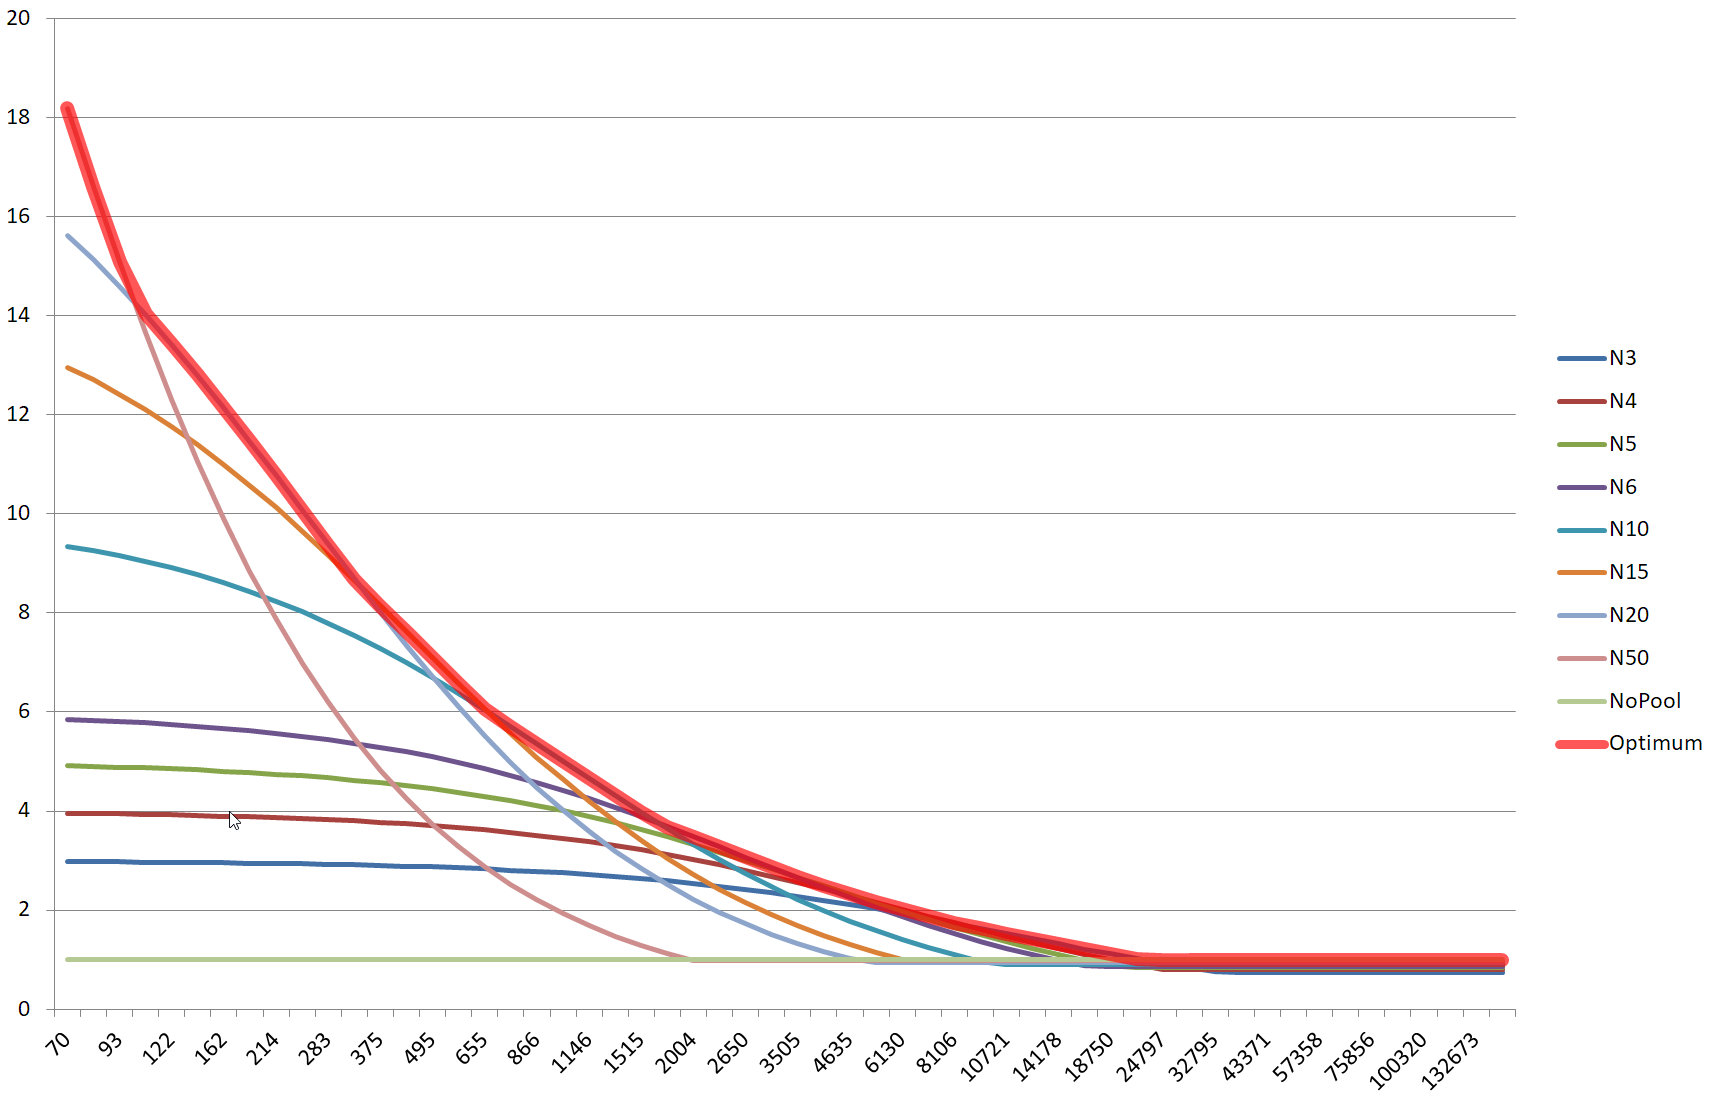
\includegraphics[height=.6\textwidth]{img/Minipool}
	%\caption{Geplanter Aufbau der Arbeit\footnotemark}
\end{figure}

\cleardoublepage

% !TEX root =  master.tex
\chapter{Analyse und Bewertung der Poolingmethoden}
\section{Qualitativ}
\cleardoublepage
\cleardoublepage

\section{Quantitativ}

\cleardoublepage
\cleardoublepage

%#########################################################
%#########################################################
\if{false}
\section{Planung aus RP}
Die Beantwortung der primären Forschungsfrage beginnt mit einer Aufbereitung der bisherigen Forschung zu PCR-Pooling-Verfahren.
Für die Validierung sind zwei Forschungsansätze denkbar:

Qualitativer Ansatz:
Die Disziplin der Kanalcodierung wird vorgestellt und auf Basis dieses wissenschaftlichen Frameworks die Pooling-Verfahren formalisiert.
Hierauf erfolgt eine argumentativ-deduktive Analyse, welche die Methode durch theoretische und qualitative Ansätze überprüft.


\section{Obsidian Sammlung}
\subsubsection{Kanalcodierung}
\begin{itemize}
	\item In der Raumfahrt ist Strahlung eines der Hauptprobleme, welche Bitflips
	\footnote{Die binäre Änderung eines Speicherfeldes}
	in Speichern auslösen kann.
	Hierbei sind oftmals Fehler inakzeptabel, weswegen hochgradig redundante Systeme zum Einsatz kommen.
	Es werden Teilweise ganze Systeme mehrfach verbaut, um die Ergebnisse zu vergleichen.
	\item Ethernetpakete haben dieselbe Herausforderung wie die Raumfahrt, dass durch Störungen Bits verloren gehen können.
	Üblicherwiese sind Ethernetpakete allerdings unkritischer, können erneut gesendet werden und die Strahlungsintensität ist geringer.
	Deshalb werden hier Fehler nur erkannt, aber auf eine Korrektur verzichtet.
	Beschädigte Pakete werden verworfen und müssen erneut gesendet werden.
	\item Anhand der existierenden RAID-Level können die unterschiedlichen Ziele von Kanalcodierung veranschaulicht werden.
	Zwischen Sicherheit, Verfügbarkeit und Berechnungsintensität muss eine Abwägung getroffen werden.
	- Ein System kann wie bei RAID-0 zulasten seiner Integrität beschleunigt werden.
	- Bei RAID-1 wird wie in der Raumfahrt eine volle Redundanz hergestellt. Die hohe Fehlertoleranz der Daten wird hierbei durch hohen Mehraufwand erkauft.
	- RAID-5 und RAID-6 versuchen die Speicherkosten zu optimieren und eine dem Umstand angemessene Datensicherheit zu erreichen. Hierbei wird ein deutlicher Berechnungsaufwand für die Parität, eine lange Rebuild-Zeit und ein gewisses Ausfallrisiko in Kauf genommen.
	\item Der Reed-Solomon-Code, welcher Beispielsweise in CDs eingesetzt wird, ist in der Lage Burst-Errors
	\footnote{Fehler, welche nicht zufällig verteilt sind, sondern in Clustern auftreten.}
	zu erkennen.
	Bei CDs kann dies der Fall sein, wenn diese durch einen zusammenhängenden Kratzer beschädigt ist.
	\item Der Hamming Code war einer der ersten ECC-Algorithmen und wurde in den 1950ern von Richard W. Hamming entwickelt.
	Seine Verteilung der Paritäts-Bits ermöglicht eine effiziente Überprüfung der Daten.
	Durch Verwendung von N+1 Paritäts-Bits, kann die Integrität von 2-hoch-N Daten zu überprüfen werden.
	Die Berichtigung einzelner Bitfehler ist ebenfalls möglich.
	Sollte mehr als ein Fehler innerhalb des Blocks auftreten, kann dieser zwar erkannt, aber nicht berichtigt werden.
	Für einen Speicherbereich mit 256 Bit werden somit 8+1 Paritäts-Bits benötigt, was einem Overhead von nur 3,5 Prozent entspricht.
	Neuere Algorithmen haben die Effizient weiter gesteigert und sollen im Laufe der Arbeit vergleichen werden.
\end{itemize}

\subsubsection{Erstellung eigener Modelle}
Geprüft werden soll die Übertragbarkeit mehrerer in der Informatik gängigen ECC-Algorithmen auf den medizinischen Bereich.
Die Theorie wäre, dass Covid-Infektionen bei anlasslosen Testungen wie auch Bitfehler selten sind.
Somit könnten dieselben Algorithmen zur Effizienzsteigerung genutzt werden.
Ziel ist es, eine Möglichkeit zu finden die exponentielle Effizienzsteigerung von ECC-Algorithmen auf medizinische Testungen anzupassen und hierdurch die Kosten deutlich zu reduzieren.
Hierbei müssen Anpassungen an den Algorithmen vorgenommen werden und neue Herausforderungen beachtet werden.

Beispielsweise sind bei einem 15-11-Hamming-Code nur 11/16 Bits echte Daten.
Die Paritätsbits kosten hier direkt Speicherkapazität.
Bei einer PCR-Testung wären theoretisch alle 16 Plätze verwendbar, da die Durchführung von PCR-Tests selbst (anders als bei Speicher) keine Plätze kostet.
Desweiteren sind neue Probleme zu erwarten, wenn die Tests von Menschen durchgeführt werden.
Hierbei entstehen Fehler, welche in den bisherigen Algorithmen keine Berücksichtigung finden mussten.


\section{Planung aus RP - Quant}
Die Beantwortung der primären Forschungsfrage beginnt mit einer Aufbereitung der bisherigen Forschung zu PCR-Pooling-Verfahren.
Für die Validierung sind zwei Forschungsansätze denkbar:

Quantitativer Ansatz:
Die Pooling-Verfahren werden in Software nachgebaut und quantitativ anhand einer Simulation analysiert.
Es werden unterschiedliche Grenzfälle getestet, um die Auswirkung auf das Verfahren zu beobachten.


\section{Obsidian Sammlung}
\fi
% !TEX root =  master.tex
\section{Betriebliche Implementierung}
Da die primäre Hypothese in Kapitel XX widerlegt wurde, entfällt die Relevanz für die Erarbeitung einer umfassenden betrieblichen Teststrategie.
Trotzdem bleibt festzuhalten, dass das PCR-Verfahren in der Schwerpunkttestung eine erhöhte Zuverlässigkeit gegenüber Schnelltests bietet.
Anstelle einer umfassenden Implementierung werden deshalb Grundsätze für die Durchführung von PCR-Pooling diskutiert.

\textbf{Pooling im Unternehmen}\newline
Das Pooling wird bei diesem Ansatz von Mitarbeitern des Unternehmens durchgeführt.
Das Labor muss nicht einmal zwangsläufig wissen, dass Pooling durchgeführt wird.
Abhängig vom Grad der Verwässerung sollte diese Information allerdings mitgeteilt werden, um die Anzahl der Zyklen zu erhöhen.

Von einer Probenverarbeitung im Unternehmen birgt mehrere Risiken, welche durch eine Auswertung im Labor vermieden werden können.

\begin{itemize}
	\item \textbf{Unsachgemäße Handhabung}\newline
	Für Mitarbeiter besteht ein Ansteckungsrisiko und die Proben könnten durch fehlerhafte Verarbeitung kontaminiert oder zerstört werden.
	\item \textbf{Effizenz}\newline
	Im Labor stehen geeignete Geräte und erfahrenes Personal zur Verfügung.
	Durch die Routine können eine höhere Geschwindigkeit und Qualität erreicht werden.
\end{itemize}

Eine Verarbeitung im Unternehmen wird deshalb grundsätzlich nicht empfohlen.
Unternehmen mit der Möglichkeit ein vollwertiges Labor einzurichten, sind hiervon ausgenommen.

\textbf{Pooling im Labor}\newline
Beim Pooling im Labor werden im Unternehmen nur die Proben entnommen, beschriftet und an das Labor gesendet.
Hierdurch wird Arbeitsaufwand an das Labor verlagert und es wird ein Labor benötigt, welches das Pooling anbietet.
Das Pooling wird hierdurch von medizinisch geschultem Personal mit angemessenen Werkzeugen durchgeführt.
Eine Durchführung des Poolings im Labor wird deshalb empfohlen.

\cleardoublepage

\textbf{Organisation im Unternehmen}\newline
Bei der Auswahl der Poolgröße muss auf die Praktikabilität von Logistik und Organisiation geachtet werden.

Bei Einführung des Systems könnte man allen Mitarbeitern Klebetiketten mit personalisiertem Barcode zusenden.
Wenn die Person an einer Testung teilnimmt, bringt sie den Codeaufkleber mit und dieser wird auf das Teströhrchen geklebt.
Die Tests werden gesammelt an das Labor gesendet und dort ausgewertet.
Zurück übermittelt werden die Testergebnisse nach Barcodenummer.
Die Ergebnisse können vom Unternehmen über die Nummer einer Person zugeordnet werden.
Personenbezogene Daten verlassen nach diesem System nicht das Unternehmen.
Zur Ermittlung von Kontaktpersonen könnten Abteilungen herangezogen werden oder die Mitarbeiter pflegen die Kontaktlisten selbst.

Die Probenentnahme muss von einer geschulten Person beaufsichtigt werden, um Fehlanwendung und Missbrauch zu verhindert.
Hierfür gibt es in vielen Betrieben bereits Personal, welches für die Beaufsichtigung der 3G-Nachweise zugelassen ist.\footnote{§XXXX}
Die Abfallmenge ließe sich durch reinigungsfähige Glasröhrchen und einen Flüssigkeitsbehälter gering halten.

\textbf{Ausstellung von Zerftikaten}\newline
In den Corona-Verordnungen wird unterschieden zwischen Schnelltests und PCR-Tests.
Mit dem Nachweis eines negativen PCR-Tests ist es möglich, zutritt zu veranstaltungen und Geschäften zu erhalten.
Der Gesetzgeber trennt hierbei klar zwischen den präzisen PCR-Tests und ungenauen Schnelltests.\footnote{Verordnung PCR Schnelltest}
Es ist anzunehmen, dass der Gesetzgeber hierbei kein oder nur ein schwaches Pooling eingerechnet hat.

Durch das Pooling großer Gruppen, könnte die Erkennungsgenauigkeit des PCR-Tests reduziert sein.
In diesen Fällen sollten nur Schnelltest-Bescheinigungen an die negativ getesteten Personen ausgestellt werden.

Test
\footcite{TD15}
\cleardoublepage

% Fazit und Ausblick
% !TEX root =  master.tex
\chapter{Ergebnis}

%#########################################################
%#########################################################
\if{false}
\section{Planung aus RP}
Die Arbeit endet mit einem Kapitel, in welchem die Erlebnisse zusammengefasst und Handlungsempfehlungen gegeben werden.
Es wird geprüft ob das Forschungsziel erreicht wurde und ob ein Optimierungspotenzial gegenüber den bisherigen Verfahren besteht.
Abhängig vom vorherigen Kapitel folgt ein Ausblick.

\section{Obsidian Notizen}
Die Arbeit endet mit einem Kapitel, in welchem die Erlebnisse zusammengefasst und Handlungsempfehlungen gegeben werden.
Es wird geprüft ob das Forschungsziel erreicht wurde und wie hoch das Optimierungspotenzial gegenüber den bisherigen Verfahren ist.
Auf dieser Basis wird ein Ausblick auf die Potenziale der betrieblichen Umsetzung gegeben.

Abhängig vom endgültigen Schwerpunkt der Arbeit, könnte die Implementierung der Verfahren ein Unterkapitel "Ausblick" im Rahmen des Ergebnisses werden.
Die Details der Implementierung würden hierdurch aus der Arbeit ausgelagert und abgegrenzt werden.
Sinnvoll könnte dies sein, wenn die primäre Forschungsfrage aufgrund von vielen unterschiedlichen Verfahren einen größeren Anteil der verfügbaren Seitenzahl beansprucht.
Die sekundäre Forschungsfrage wird somit flexibel angepasst, um ausreichend Ressourcen für die primäre Forschungsfrage bereitzustellen.

\subsection{Known Issues}
A) Tagesaktuelle Veränderung der Lage. Aged like Milk.
A2) Probleme bei der wissenschaftlichkeit einiger Passagen.

B) Man bescheinigt Leuten ein PCR-Negativergebnis, für die 3/4 Tests positiv waren.
- Risiko / Fehlerquote
- Verunsicherung
- Nachprüfung und resultierende Kosten

C) Fehler von PCR-Tests / Akzeptable Quote

D) Mögliche Anwendungsfehler

E) XOR / AND bei Algorithmen
Mitigation
A) Veraltung

Tagesaktuelle Lage wird beschrieben und eingeordnet.
Verankerung und Dokumentation im aktuellen Zeitgeschehen
Andere Komponente ist jahrzehnte alt und erprobt. Keine Veränderung.
Methodik kann für weitere Erkrankungen genutzt werden
PCR-Covid19-Tests dürften noch eine Weile erhalten bleiben. Unabhängig der exakten Lage
B) Fehlerquote

Berücksichtigung innerhalb der Konzipierung
Organisatorische Minimierung
\fi


%%%%%%%%%%%%%%%%%%%%%%%%%%%%%%%%%%%
%% !TEX root =  master.tex
\chapter{Quellenarbeit}

\section{Verwilt / prePrint / Vier Versionen}
https://www.medrxiv.org/content/10.1101/2020.07.17.20152702v4


\section{Calabrese / prePrint / Zwei Versionen}
https://www.medrxiv.org/content/10.1101/2020.12.21.20248431v2


\section{Viehweger / prePrint / Zwei Versionen}
https://www.medrxiv.org/content/10.1101/2020.04.16.20067603v2

Primärquellen in Zeile 24

Prevalence = Inzidenz / Anteil Infizierter in Population

Developed "Clonepool" - a software to calculate the Pool layouts under a BSD license https://github.com/phiweger/clonepool


11 when a traditional pool is tested positive, all samples in the pool need individual retesting, which becomes
12 ineffective at a higher proportion of positive samples.

14 At 2 Percent prevalence and 20 samples
15 per pool, our protocol increases screening capacity by factors of 5 and 2 compared to individual testing
16 and traditional pooling, respectively.

21 In most
22 laboratories, the screening capacity is limited by the number of PCR reactions that can be performed in
23 a day. It is, therefore, desirable to maximize the number of samples that can be tested per reaction.

27 A high prevalence renders traditional pooling ineffective.

50 We tested the proposed clonepool algorithm using simulated data. We assumed no pipetting errors,
51 which can be achieved, e.g., through the use of a pipetting robot. We also assume that 94 pools are
52 available, which corresponds to a 96-well plate with two wells reserved for a positive and a negative
53 control. Furthermore, we assume that there are no false positive or false negative PCR reactions.

61 The number of samples that can be pooled without affecting the PCR sensitivity is limited by the PCR
62 cycle threshold (Ct) for the target, i.e., the cycle at which amplification becomes detectable over back
63 ground noise (typically ten times the standard deviation, SD). Usually, Ct values above 35 are treated
64 as unspecific amplification. SARS-CoV-2 amplifies at low Ct values due to high viral titers (Ct 18-25
65 depending on the material and number of days post-infection).4,5 A 20-fold dilution, i.e., pooling 20 sam-
66 ples, would cause the Ct value to increase by about 4.3 cycles (2𝑥 = 𝑑, where d is the dilution and x the
67 shift in Ct), which still lies comfortably above the detection limit.

%%%%%%%%%%%%%%%%%%%%%%%%%%%%%%%%%%%
% LITERATURVERZEICHNIS
% @stud: Literaturverzeichnis in Datei bibliography.bib anpassen. 
%
% Alternative zu Verwendung von \initializeBibliography: Citavi ...
% (dann \initializeBibliography auskommentieren und eigenes LaTex Coding verwenden)
%
%\ihead{}
\printbibliography[title=\Literaturverzeichnis] 
\cleardoublepage
% Kopiert aus Config
%%%%%%%%%%%%%%%%%%%%%%%%%%%%%%%%%%%

%%%%%%%%%%%%%%%%%%%%%%%%%%%%%%%%%%%
% ANHÄNGE
%
% @stud: einzelne Anhänge bearbeiten und eigene Anhänge hier einfügen 
%        die nachfolgenden Zeilen deaktivieren, wenn keine Anhänge verwendet werden
%
%\initializeAppendix
% !TEX root =  master.tex
\chapter{Tabelle Optimale Testgrößen}
\begin{figure}[h]
	\centering
	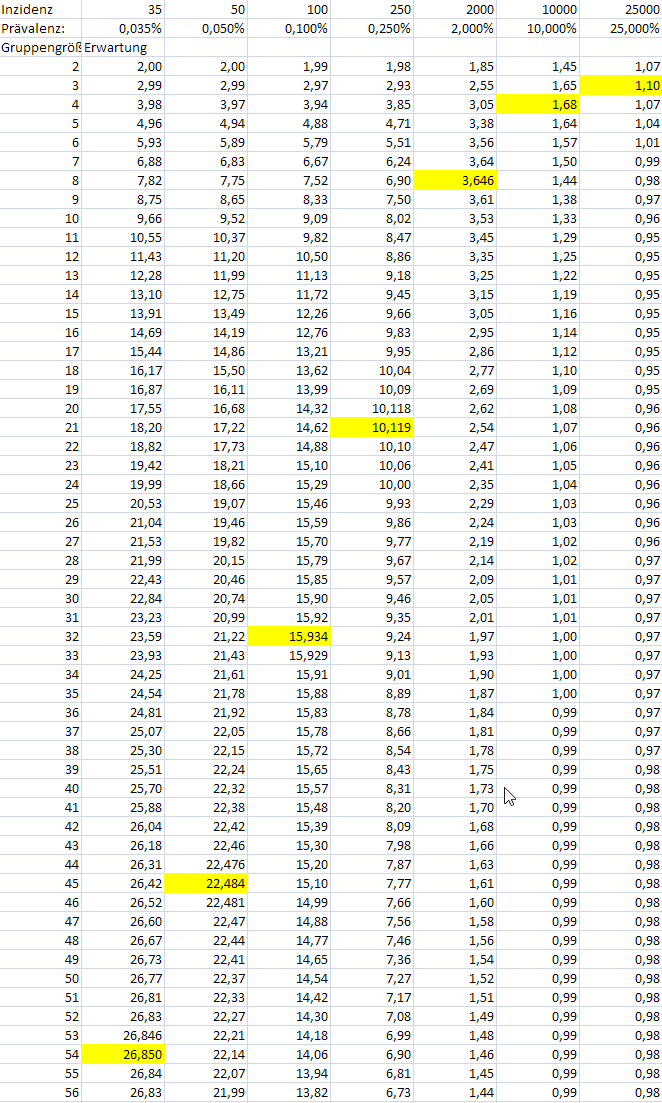
\includegraphics[width=.63\textwidth]{img/TabelleOptimum}
	\caption{Tabelle Optimale Testgrößen\footnotemark}
\end{figure}
\footnotetext{Eigene Darstellung}

%% !TEX root =  master.tex
\chapter{Beispiel-Anhang: Noch ein Testanhang}
nochmal: lipsum ...

%%%%%%%%%%%%%%%%%%%%%%%%%%%%%%%%%%%

%\singlespacing

%%%%%%%%%%%%%%%%%%%%%%%%%%%%%%%%%%%
% INDEX
% @stud: ggf. Index auskommentieren, wenn nicht benötigt
%
%\addcontentsline{toc}{chapter}{Index}
%\printindex

\end{document}
